
\chapter{经典CNN架构——从LeNet到ResNet}

\intro{CNN的发展史是一部精妙的工程进化史：LeNet-5在1998年定义了卷积+池化+全连接的基本范式；AlexNet在2012年开启了深度学习时代；VGG证明了深度的力量；GoogLeNet引入了多尺度特征融合；ResNet用残差连接突破了深度瓶颈。本章按时间顺序逐一解析这些里程碑架构，理解每项创新背后的"为什么"。}

%%%%%%%%%%%%%%%%%%%%%%%%%%%%%%%%%%%%%%%%%%%%%%%%%%%%%%%%
\section{LeNet-5——CNN的起源（1998年）}

LeNet-5由Yann LeCun于1998年提出，用于手写数字识别（MNIST）。虽然只有约6万个参数，但它奠定了CNN的基本架构范式。

\begin{figure}[H]\centering
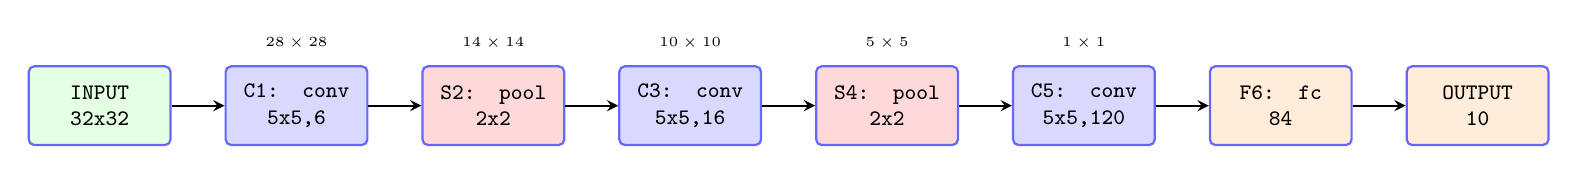
\begin{tikzpicture}[
    myblock/.style={rectangle, draw=blue!60, thick, fill=blue!5, minimum width=1.8cm, minimum height=1.0cm, font=\footnotesize\ttfamily, rounded corners=2pt, align=center},
    myarrow/.style={->, >=stealth, thick},
]
\node[myblock, fill=green!10] (inp) at (0,0) {INPUT\\32x32};
\node[myblock, fill=blue!15] (c1)  at (2.5,0) {C1: conv\\5x5,6};
\node[myblock, fill=red!15] (s2)  at (5.0,0) {S2: pool\\2x2};
\node[myblock, fill=blue!15] (c3)  at (7.5,0) {C3: conv\\5x5,16};
\node[myblock, fill=red!15] (s4)  at (10.0,0) {S4: pool\\2x2};
\node[myblock, fill=blue!15] (c5)  at (12.5,0) {C5: conv\\5x5,120};
\node[myblock, fill=orange!15] (f6) at (15.0,0) {F6: fc\\84};
\node[myblock, fill=orange!15] (out) at (17.5,0) {OUTPUT\\10};

\draw[myarrow] (inp) -- (c1);
\draw[myarrow] (c1) -- (s2);
\draw[myarrow] (s2) -- (c3);
\draw[myarrow] (c3) -- (s4);
\draw[myarrow] (s4) -- (c5);
\draw[myarrow] (c5) -- (f6);
\draw[myarrow] (f6) -- (out);

\node[font=\tiny] at (2.5,0.8) {$28\times28$};
\node[font=\tiny] at (5.0,0.8) {$14\times14$};
\node[font=\tiny] at (7.5,0.8) {$10\times10$};
\node[font=\tiny] at (10.0,0.8) {$5\times5$};
\node[font=\tiny] at (12.5,0.8) {$1\times1$};
\end{tikzpicture}
\caption{LeNet-5的架构。卷积和池化交替，最后接全连接层。这个经典范式影响了此后所有CNN的设计}
\label{fig:lenet5}
\end{figure}

LeNet-5的核心设计元素：
\begin{itemize}
    \item \textbf{交替的卷积与池化}——Conv $\to$ Pool $\to$ Conv $\to$ Pool $\to$ FC，逐步降低空间分辨率并提取高层次特征
    \item \textbf{局部感受野}——每个隐藏神经元只连接输入的一个小邻域
    \item \textbf{参数共享}——同一卷积核在整个输入上共享参数
    \item \textbf{输出层使用欧氏径向基函数}（RBF）而非Softmax（后已被Softmax替代）
\end{itemize}

\begin{mycode}{PyTorch 实现 LeNet-5}
\begin{lstlisting}[language=Python]
import torch.nn as nn
import torch.nn.functional as F

class LeNet5(nn.Module):
    def __init__(self, num_classes=10):
        super().__init__()
        # 卷积部�?        self.conv1 = nn.Conv2d(1, 6, kernel_size=5)
        self.pool1 = nn.MaxPool2d(kernel_size=2, stride=2)
        self.conv2 = nn.Conv2d(6, 16, kernel_size=5)
        self.pool2 = nn.MaxPool2d(kernel_size=2, stride=2)
        self.conv3 = nn.Conv2d(16, 120, kernel_size=5)

        # 全连接部�?        self.fc1 = nn.Linear(120, 84)
        self.fc2 = nn.Linear(84, num_classes)

    def forward(self, x):
        x = self.pool1(F.relu(self.conv1(x)))   # -> 6x14x14
        x = self.pool2(F.relu(self.conv2(x)))   # -> 16x5x5
        x = F.relu(self.conv3(x))                # -> 120x1x1
        x = x.view(x.size(0), -1)               # 展平
        x = F.relu(self.fc1(x))                  # -> 84
        x = self.fc2(x)                          # -> 10
        return x

model = LeNet5(num_classes=10)
# 测试前向传播
import torch
x = torch.randn(1, 1, 32, 32)
out = model(x)
print(f"LeNet-5: {x.shape} -> {out.shape}")
print(f"参数量: {sum(p.numel() for p in model.parameters()):,}")
\end{lstlisting}
\end{mycode}

LeNet-5的局限：网络较浅（仅3层卷积），激活函数使用Sigmoid/Tanh（非ReLU），没有BatchNorm和Dropout，仅适用于MNIST级别的小规模任务。

%%%%%%%%%%%%%%%%%%%%%%%%%%%%%%%%%%%%%%%%%%%%%%%%%%%%%%%%
\section{AlexNet——深度学习革命的起点（2012年）}

AlexNet在2012年ImageNet竞赛中以top-5错误率15.3\%夺冠（当年第二名26.2\%），标志了深度学习视觉时代的正式开启。

AlexNet相比LeNet-5的革命性创新：
\begin{itemize}
    \item \textbf{首次使用ReLU}——将训练速度提升了数倍，并缓解了梯度消失
    \item \textbf{双GPU并行训练}——网络分两半部署在两块GTX 580 GPU上（当时显存仅3GB）
    \item \textbf{重叠池化}（Overlapping Pooling）——$3\times3$窗口，步长2，比不重叠的$2\times2$稍有改进
    \item \textbf{局部响应归一化}（LRN）——模拟了生物神经元的侧抑制，但后来被BatchNorm取代
    \item \textbf{Dropout}——首次应用于全连接层，有效缓解过拟合
    \item \textbf{数据增强}——随机裁剪和水平翻转，增加训练数据的多样性
\end{itemize}

\begin{figure}[H]\centering
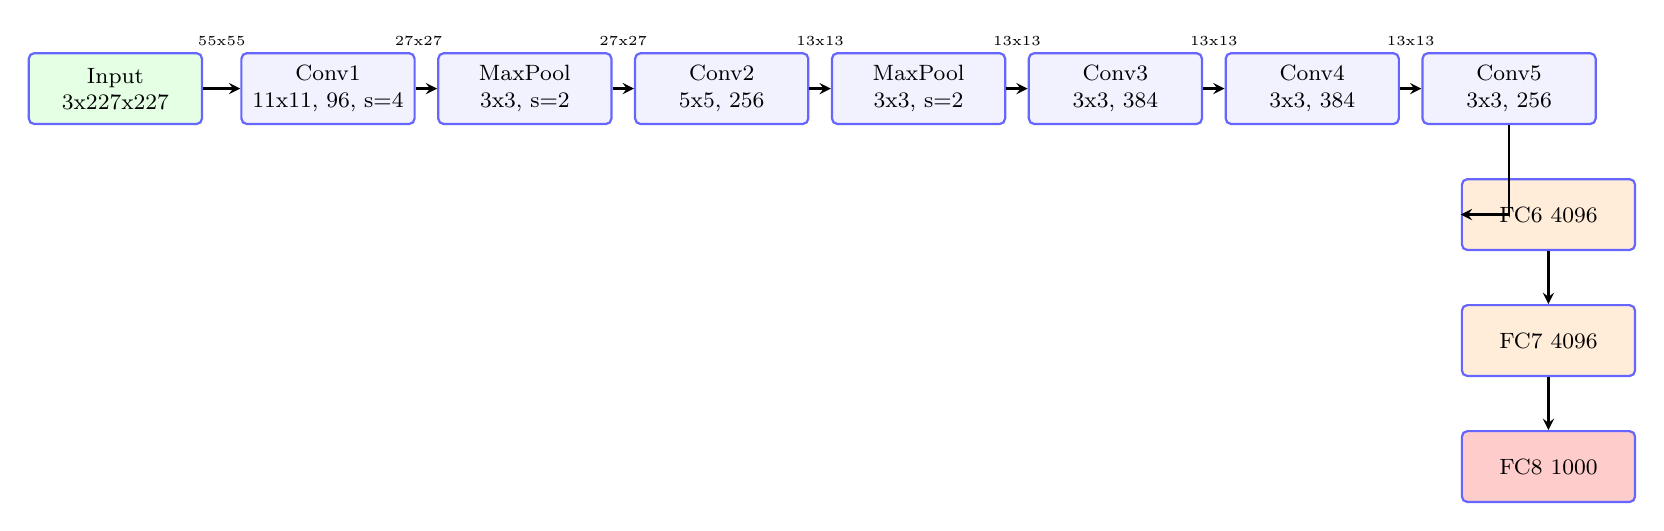
\begin{tikzpicture}[
    myblock/.style={rectangle, draw=blue!60, thick, fill=blue!5, minimum width=2.2cm, minimum height=0.9cm, font=\footnotesize, rounded corners=2pt, align=center},
    myarrow/.style={->, >=stealth, thick},
]
\node[myblock, fill=green!10] (inp) at (0,0) {Input\\3x227x227};
\node[myblock] (c1)  at (2.7,0) {Conv1\\11x11, 96, s=4};
\node[myblock] (p1)  at (5.2,0) {MaxPool\\3x3, s=2};
\node[myblock] (c2)  at (7.7,0) {Conv2\\5x5, 256};
\node[myblock] (p2)  at (10.2,0) {MaxPool\\3x3, s=2};
\node[myblock] (c3)  at (12.7,0) {Conv3\\3x3, 384};
\node[myblock] (c4)  at (15.2,0) {Conv4\\3x3, 384};
\node[myblock] (c5)  at (17.7,0) {Conv5\\3x3, 256};
\node[myblock, fill=orange!15] (ta) at (18.2,-1.6) {FC6 4096};
\node[myblock, fill=orange!15] (tb) at (18.2,-3.2) {FC7 4096};
\node[myblock, fill=red!20] (tc) at (18.2,-4.8) {FC8 1000};

\draw[myarrow] (inp) -- (c1);
\draw[myarrow] (c1) -- (p1);
\draw[myarrow] (p1) -- (c2);
\draw[myarrow] (c2) -- (p2);
\draw[myarrow] (p2) -- (c3);
\draw[myarrow] (c3) -- (c4);
\draw[myarrow] (c4) -- (c5);
\draw[myarrow] (c5) |- (ta);
\draw[myarrow] (ta) -- (tb);
\draw[myarrow] (tb) -- (tc);

\node[font=\tiny] at (1.35,0.6) {55x55};
\node[font=\tiny] at (3.85,0.6) {27x27};
\node[font=\tiny] at (6.45,0.6) {27x27};
\node[font=\tiny] at (8.95,0.6) {13x13};
\node[font=\tiny] at (11.45,0.6) {13x13};
\node[font=\tiny] at (13.95,0.6) {13x13};
\node[font=\tiny] at (16.45,0.6) {13x13};
\end{tikzpicture}
\caption{AlexNet的架构。5层卷积（前两层带池化）+ 3层全连接。首次使用了ReLU和Dropout}
\label{fig:alexnet}
\end{figure}

参数分布：AlexNet约6000万参数，其中全连接层（FC6和FC7）占总参数的90\%以上。这一事实直接催生了后续架构的一个设计趋势——减少甚至消除全连接层。

%%%%%%%%%%%%%%%%%%%%%%%%%%%%%%%%%%%%%%%%%%%%%%%%%%%%%%%%
\section{VGG——深度的重要性（2014年）}

牛津大学VGG组在2014年做出的关键贡献不是架构上的新花样，而是\textbf{极致的统一与深度}：

\begin{itemize}
    \item 所有卷积层使用统一的 $3\times3$ 卷积核（最小的非平凡尺寸）
    \item 池化层使用统一的 $2\times2$ 最大池化，步长2
    \item 每次池化后通道数翻倍（64 $\to$ 128 $\to$ 256 $\to$ 512 $\to$ 512）
    \item 通过堆叠层数控制模型容量：VGG-16（16层）和VGG-19（19层）
\end{itemize}

\begin{myTheorem}{VGG的设计原理}
两个 $3\times3$ 卷积堆叠的感受野等价于一个 $5\times5$ 卷积，三个 $3\times3$ 堆叠等价于一个 $7\times7$。但使用小核堆叠的好处是：(1) 参数更少；(2) 中间有更多ReLU，增加非线性；(3) 计算效率更高。
\end{myTheorem}

VGG的主要缺点：
\begin{itemize}
    \item \textbf{参数巨大}——VGG-16有1.38亿参数，其中约1.2亿在全连接层
    \item \textbf{内存消耗大}——前两个FC层需要470MB的存储
    \item \textbf{计算开销高}——大量通道导致中间特征图占用大量显存
\end{itemize}

尽管存在这些缺点，VGG的简单性和统一性使其成为特征提取的首选骨干网络（backbone），其预训练权重至今仍广泛用于风格迁移、图像生成等任务中。

%%%%%%%%%%%%%%%%%%%%%%%%%%%%%%%%%%%%%%%%%%%%%%%%%%%%%%%%
\section{GoogLeNet / Inception——多尺度特征融合（2014年）}

GoogLeNet（与VGG同年）从另一个方向解决了深度网络的挑战：不再追求更深的堆叠，而是\textbf{在每一层内并行使用不同尺寸的卷积核}，而后将这些多尺度特征拼接。

\subsection{Inception模块}

Inception模块的核心思想：网络不必在每一层决定使用哪种尺寸的卷积核，而是让网络自己学习——并行地使用$1\times1$、$3\times3$和$5\times5$卷积以及$3\times3$最大池化，然后将所有分支的输出在通道维度上拼接。

\begin{figure}[H]\centering
\begin{tikzpicture}[
    myblock/.style={rectangle, draw=blue!60, thick, fill=blue!5, minimum width=2.0cm, minimum height=0.7cm, font=\footnotesize, rounded corners=2pt, align=center},
    myarrow/.style={->, >=stealth, thick},
    node distance=0.4cm,
]
\node[myblock] (prev) at (0,0) {前一层};

\node[myblock, fill=red!10] (c1x1_a) at (3.5,1.8) {Conv\\1x1};
\node[myblock, fill=orange!10] (c3x3_r) at (3.5,0.6) {Conv\\1x1 reduce};
\node[myblock, fill=orange!10] (c3x3)   at (6.0,0.6) {Conv\\3x3};
\node[myblock, fill=green!10] (c5x5_r) at (3.5,-0.6) {Conv\\1x1 reduce};
\node[myblock, fill=green!10] (c5x5)   at (6.0,-0.6) {Conv\\5x5};
\node[myblock, fill=blue!10]  (pool)   at (3.5,-1.8) {MaxPool\\3x3};
\node[myblock, fill=blue!10]  (pool1)  at (6.0,-1.8) {Conv\\1x1};

\node[myblock, fill=violet!15] (concat) at (9.0,0) {拼接};

\draw[myarrow] (prev) -- (c1x1_a);
\draw[myarrow] (prev) -- (c3x3_r);
\draw[myarrow] (prev) -- (c5x5_r);
\draw[myarrow] (prev) -- (pool);
\draw[myarrow] (c1x1_a) -- (concat);
\draw[myarrow] (c3x3_r) -- (c3x3);
\draw[myarrow] (c3x3) -- (concat);
\draw[myarrow] (c5x5_r) -- (c5x5);
\draw[myarrow] (c5x5) -- (concat);
\draw[myarrow] (pool) -- (pool1);
\draw[myarrow] (pool1) -- (concat);

\node[font=\tiny, red!70!black] at (3.5,2.3) {直接1x1分支};
\node[font=\tiny, orange!70!black] at (5.0,1.1) {降维后3x3分支};
\node[font=\tiny, green!70!black] at (5.0,-1.1) {降维后5x5分支};
\node[font=\tiny, blue!70!black] at (5.0,-2.3) {池化+1x1分支};
\end{tikzpicture}
\caption{Inception模块（带降维的版本）。$1\times1$卷积在$3\times3$和$5\times5$卷积前降维，大幅减少计算量。$1\times1$卷积是Inception经济的秘密}
\label{fig:inception-module}
\end{figure}

\subsection{辅助分类器}

GoogLeNet在中间层添加了两个辅助分类器（auxiliary classifiers），将中间层的特征也用于分类并计算损失，提供额外的梯度信号来对抗深层网络的梯度消失。这些辅助分类器在推理时被丢弃。

\begin{mycode}{简化版 Inception 模块的 PyTorch 实现}
\begin{lstlisting}[language=Python]
import torch
import torch.nn as nn

class InceptionModule(nn.Module):
    def __init__(self, in_channels, out_1x1,
                 red_3x3, out_3x3,
                 red_5x5, out_5x5, out_pool):
        super().__init__()
        # 1x1 分支
        self.branch1 = nn.Sequential(
            nn.Conv2d(in_channels, out_1x1, 1),
            nn.BatchNorm2d(out_1x1),
            nn.ReLU(inplace=True)
        )
        # 1x1 -> 3x3 分支
        self.branch2 = nn.Sequential(
            nn.Conv2d(in_channels, red_3x3, 1),
            nn.BatchNorm2d(red_3x3),
            nn.ReLU(inplace=True),
            nn.Conv2d(red_3x3, out_3x3, 3, padding=1),
            nn.BatchNorm2d(out_3x3),
            nn.ReLU(inplace=True)
        )
        # 1x1 -> 5x5 分支（常替�? 两个3x3�?
        self.branch3 = nn.Sequential(
            nn.Conv2d(in_channels, red_5x5, 1),
            nn.BatchNorm2d(red_5x5),
            nn.ReLU(inplace=True),
            nn.Conv2d(red_5x5, out_5x5, 3, padding=1),
            nn.BatchNorm2d(out_5x5),
            nn.ReLU(inplace=True),
            nn.Conv2d(out_5x5, out_5x5, 3, padding=1),
            nn.BatchNorm2d(out_5x5),
            nn.ReLU(inplace=True)
        )
        # 池化分�?        self.branch4 = nn.Sequential(
            nn.MaxPool2d(3, stride=1, padding=1),
            nn.Conv2d(in_channels, out_pool, 1),
            nn.BatchNorm2d(out_pool),
            nn.ReLU(inplace=True)
        )

    def forward(self, x):
        b1 = self.branch1(x)
        b2 = self.branch2(x)
        b3 = self.branch3(x)
        b4 = self.branch4(x)
        return torch.cat([b1, b2, b3, b4], dim=1)

# 测试
x = torch.randn(2, 256, 14, 14)
module = InceptionModule(256, 64, 96, 128, 16, 32, 32)
out = module(x)
print(f"Inception: {x.shape} -> {out.shape}")
\end{lstlisting}
\end{mycode}

%%%%%%%%%%%%%%%%%%%%%%%%%%%%%%%%%%%%%%%%%%%%%%%%%%%%%%%%
\section{ResNet——残差网络，突破深度极限（2015年）}

\subsection{退化问题}

VGG证明了增加深度可以提升性能。但实验发现：当网络深度超过某个阈值后，训练误差和测试误差反而上升——这不是过拟合，而是\textbf{退化}（degradation）。理论上，更深的网络至少不应该比浅层网络更差（深层网络的后几层可以学习恒等映射，退化为浅层网络）。然而，SGD难以学习恒等映射。

\subsection{残差学习——Let the layers fit a residual mapping}

ResNet的核心洞察：与其让层直接学习期望映射 $\mathcal{H}(\mathbf{x})$，不如让层学习\textbf{残差} $\mathcal{F}(\mathbf{x}) = \mathcal{H}(\mathbf{x}) - \mathbf{x}$。最终输出为 $\mathcal{H}(\mathbf{x}) = \mathcal{F}(\mathbf{x}) + \mathbf{x}$。

如果恒等映射是最优的，优化器只需将残差分支的权重推向零即可（比学习恒等映射容易得多）。

\begin{figure}[H]\centering
\begin{tikzpicture}[
    myblock/.style={rectangle, draw=blue!60, thick, fill=blue!5, minimum width=2.0cm, minimum height=0.8cm, font=\footnotesize, rounded corners=2pt},
    myarrow/.style={->, >=stealth, thick},
]
\node[myblock] (x) at (0,0) {$\mathbf{x}$};

\node[myblock] (w1) at (3,1.2) {权重层};
\node[myblock] (relu1) at (5.5,1.2) {ReLU};
\node[myblock] (w2) at (8,1.2) {权重层};

\draw[myarrow] (x.east) -- (1.5,0) |- (w1.west);
\draw[myarrow] (w1.east) -- (relu1.west);
\draw[myarrow] (relu1.east) -- (w2.west);

\draw[myarrow, blue!60, line width=1.5pt] (x.east) -- (11,0) --
    (11,0) -| (9.5,1.2);

\node[draw=orange!80, circle, thick, fill=orange!10, minimum size=0.6cm, font=\footnotesize] at (9.5,1.2) {$+$};
\node[myblock] (relu2) at (11.5,1.2) {ReLU};
\draw[myarrow] (w2.east) -- (9.5,1.2);
\draw[myarrow] (9.5,0.9) -- (relu2.west);

\node[font=\small\bfseries, blue!60] at (5.5,-0.6) {$\mathcal{F}(\mathbf{x})$};
\node[font=\small\bfseries, blue!60] at (11,-0.6) {$\mathcal{F}(\mathbf{x}) + \mathbf{x}$};
\node[font=\footnotesize, blue!70] at (5.5,-1.1) {残差映射};
\node[font=\footnotesize, blue!70] at (11,-1.1) {跳跃连接（identity）};

% \node[font=\footnotesize, anchor=west] at (13.0,0) {输出 = $\mathcal{F}(\mathbf{x}) + \mathbf{x}$};
\end{tikzpicture}
\caption{残差块（Residual Block）的结构。跳跃连接（shortcut connection）将输入$\mathbf{x}$直接加到残差分支的输出上，使得梯度可以通过这条"高速公路"无损地传递到浅层}
\label{fig:residual-block}
\end{figure}

\subsection{残差连接解决梯度消失}

对于残差块 $\mathbf{y} = \mathcal{F}(\mathbf{x}, \{W_i\}) + \mathbf{x}$，反向传播时梯度为：

\[
\frac{\partial \mathcal{L}}{\partial \mathbf{x}} = \frac{\partial \mathcal{L}}{\partial \mathbf{y}} \cdot \left(\frac{\partial \mathcal{F}}{\partial \mathbf{x}} + \mathbf{I}\right)
\]

单位矩阵 $\mathbf{I}$ 的存在保证了梯度至少有一条直接的通路到达任意浅层——即使 $\partial \mathcal{F}/\partial \mathbf{x}$ 很小，梯度也不会完全消失。这是ResNet能够训练152层甚至1000+层网络的根本原因。

\subsection{Bottleneck残差块}

对于极深网络（ResNet-50/101/152），使用\textbf{bottleneck}结构减少计算量：

\[
\text{Conv1x1}(C_{\text{in}} \to C_{\text{mid}}) \to \text{Conv3x3}(C_{\text{mid}} \to C_{\text{mid}}) \to \text{Conv1x1}(C_{\text{mid}} \to C_{\text{out}})
\]

其中 $C_{\text{mid}} = C_{\text{out}} / 4$。$1\times1$卷积先降维再升维，使得$3\times3$卷积在低维空间执行，大幅减少参数量和计算量。

\begin{mycode}{ResNet 残差块和完整网络的 PyTorch 实现}
\begin{lstlisting}[language=Python]
import torch
import torch.nn as nn

class BasicBlock(nn.Module):
    """ResNet-18/34 的残差块"""
    expansion = 1

    def __init__(self, in_channels, out_channels,
                 stride=1, downsample=None):
        super().__init__()
        self.conv1 = nn.Conv2d(in_channels, out_channels,
                               3, stride, 1, bias=False)
        self.bn1 = nn.BatchNorm2d(out_channels)
        self.conv2 = nn.Conv2d(out_channels, out_channels,
                               3, 1, 1, bias=False)
        self.bn2 = nn.BatchNorm2d(out_channels)
        self.downsample = downsample
        self.relu = nn.ReLU(inplace=True)

    def forward(self, x):
        identity = x

        out = self.relu(self.bn1(self.conv1(x)))
        out = self.bn2(self.conv2(out))

        if self.downsample is not None:
            identity = self.downsample(x)

        out += identity
        out = self.relu(out)
        return out

class Bottleneck(nn.Module):
    """ResNet-50/101/152 的 Bottleneck 残差块"""
    expansion = 4

    def __init__(self, in_channels, out_channels,
                 stride=1, downsample=None):
        super().__init__()
        mid_channels = out_channels

        self.conv1 = nn.Conv2d(in_channels, mid_channels,
                               1, bias=False)
        self.bn1 = nn.BatchNorm2d(mid_channels)
        self.conv2 = nn.Conv2d(mid_channels, mid_channels,
                               3, stride, 1, bias=False)
        self.bn2 = nn.BatchNorm2d(mid_channels)
        self.conv3 = nn.Conv2d(mid_channels,
                               out_channels * self.expansion,
                               1, bias=False)
        self.bn3 = nn.BatchNorm2d(
            out_channels * self.expansion)
        self.relu = nn.ReLU(inplace=True)
        self.downsample = downsample

    def forward(self, x):
        identity = x

        out = self.relu(self.bn1(self.conv1(x)))
        out = self.relu(self.bn2(self.conv2(out)))
        out = self.bn3(self.conv3(out))

        if self.downsample is not None:
            identity = self.downsample(x)

        out += identity
        out = self.relu(out)
        return out

class ResNet(nn.Module):
    """通用的 ResNet 实现"""
    def __init__(self, block, layers, num_classes=1000):
        super().__init__()
        self.in_channels = 64

        # Stem: 初始卷积�?        self.conv1 = nn.Conv2d(3, 64, 7, stride=2,
                               padding=3, bias=False)
        self.bn1 = nn.BatchNorm2d(64)
        self.relu = nn.ReLU(inplace=True)
        self.maxpool = nn.MaxPool2d(3, stride=2, padding=1)

        # ResNet 主体
        self.layer1 = self._make_layer(
            block, 64, layers[0])
        self.layer2 = self._make_layer(
            block, 128, layers[1], stride=2)
        self.layer3 = self._make_layer(
            block, 256, layers[2], stride=2)
        self.layer4 = self._make_layer(
            block, 512, layers[3], stride=2)

        # 分类头
        self.avgpool = nn.AdaptiveAvgPool2d((1, 1))
        self.fc = nn.Linear(512 * block.expansion,
                            num_classes)

    def _make_layer(self, block, out_channels,
                    blocks, stride=1):
        downsample = None
        if stride != 1 or \
           self.in_channels != out_channels * block.expansion:
            downsample = nn.Sequential(
                nn.Conv2d(self.in_channels,
                          out_channels * block.expansion,
                          1, stride, bias=False),
                nn.BatchNorm2d(
                    out_channels * block.expansion)
            )

        layers = []
        layers.append(
            block(self.in_channels, out_channels,
                  stride, downsample)
        )
        self.in_channels = out_channels * block.expansion

        for _ in range(1, blocks):
            layers.append(
                block(self.in_channels, out_channels)
            )

        return nn.Sequential(*layers)

    def forward(self, x):
        x = self.relu(self.bn1(self.conv1(x)))
        x = self.maxpool(x)

        x = self.layer1(x)
        x = self.layer2(x)
        x = self.layer3(x)
        x = self.layer4(x)

        x = self.avgpool(x)
        x = torch.flatten(x, 1)
        x = self.fc(x)
        return x

# ========== 各版本 ResNet ==========
def resnet18(num_classes=1000):
    return ResNet(BasicBlock, [2,2,2,2], num_classes)

def resnet34(num_classes=1000):
    return ResNet(BasicBlock, [3,4,6,3], num_classes)

def resnet50(num_classes=1000):
    return ResNet(Bottleneck, [3,4,6,3], num_classes)

def resnet101(num_classes=1000):
    return ResNet(Bottleneck, [3,4,23,3], num_classes)

def resnet152(num_classes=1000):
    return ResNet(Bottleneck, [3,8,36,3], num_classes)

# 测试
model = resnet50(num_classes=10)
x = torch.randn(2, 3, 224, 224)
out = model(x)
print(f"ResNet-50: {x.shape} -> {out.shape}")
print(f"参数量: {sum(p.numel() for p in model.parameters()):,}")
\end{lstlisting}
\end{mycode}

\subsection{ResNet 架构配置表}

\begin{center}
\begin{tabular}{c|cccc}
\toprule
\textbf{层名} & \textbf{ResNet-18} & \textbf{ResNet-34} & \textbf{ResNet-50} & \textbf{ResNet-152} \\
\midrule
conv1 & \multicolumn{4}{c}{$7\times7$, 64, stride 2} \\
\multicolumn{5}{c}{$3\times3$ max pool, stride 2} \\
\midrule
conv2\_x & $\begin{bmatrix}3\times3,64\\3\times3,64\end{bmatrix}\times 2$ &
$\begin{bmatrix}3\times3,64\\3\times3,64\end{bmatrix}\times 3$ &
$\begin{bmatrix}1\times1,64\\3\times3,64\\1\times1,256\end{bmatrix}\times 3$ &
$\begin{bmatrix}1\times1,64\\3\times3,64\\1\times1,256\end{bmatrix}\times 3$ \\[8pt]
conv3\_x & $\begin{bmatrix}3\times3,128\\3\times3,128\end{bmatrix}\times 2$ &
$\begin{bmatrix}3\times3,128\\3\times3,128\end{bmatrix}\times 4$ &
$\begin{bmatrix}1\times1,128\\3\times3,128\\1\times1,512\end{bmatrix}\times 4$ &
$\begin{bmatrix}1\times1,128\\3\times3,128\\1\times1,512\end{bmatrix}\times 8$ \\[8pt]
conv4\_x & $\begin{bmatrix}3\times3,256\\3\times3,256\end{bmatrix}\times 2$ &
$\begin{bmatrix}3\times3,256\\3\times3,256\end{bmatrix}\times 6$ &
$\begin{bmatrix}1\times1,256\\3\times3,256\\1\times1,1024\end{bmatrix}\times 6$ &
$\begin{bmatrix}1\times1,256\\3\times3,256\\1\times1,1024\end{bmatrix}\times 36$ \\[8pt]
conv5\_x & $\begin{bmatrix}3\times3,512\\3\times3,512\end{bmatrix}\times 2$ &
$\begin{bmatrix}3\times3,512\\3\times3,512\end{bmatrix}\times 3$ &
$\begin{bmatrix}1\times1,512\\3\times3,512\\1\times1,2048\end{bmatrix}\times 3$ &
$\begin{bmatrix}1\times1,512\\3\times3,512\\1\times1,2048\end{bmatrix}\times 3$ \\[8pt]
\midrule
输出 & \multicolumn{4}{c}{average pool, 1000-d fc, softmax} \\
\midrule
\textbf{参数量} & 11.7M & 21.8M & 25.6M & 60.2M \\
\bottomrule
\end{tabular}
\end{center}

%%%%%%%%%%%%%%%%%%%%%%%%%%%%%%%%%%%%%%%%%%%%%%%%%%%%%%%%
\section{DenseNet——连接一切（2017年）}

DenseNet将ResNet的``跳跃连接''思想推向极致：每一层的输出都连接到\textbf{所有后续层}的输入。对于第 $l$ 层：

\[
\mathbf{x}_l = H_l([\mathbf{x}_0, \mathbf{x}_1, \mathbf{x}_2, \dots, \mathbf{x}_{l-1}])
\]

其中 $[\cdots]$ 表示在通道维度上拼接（而非相加）。这一设计带来了三个关键优势：
\begin{itemize}
    \item \textbf{减轻梯度消失}——所有层直接接收来自损失函数的监督信号
    \item \textbf{特征重用}——浅层特征被所有后续层直接使用，无需逐层传递
    \item \textbf{大幅减少参数}——由于特征重用，每层的输出通道数可以很小（12或32），总参数量反而少于ResNet
\end{itemize}

%%%%%%%%%%%%%%%%%%%%%%%%%%%%%%%%%%%%%%%%%%%%%%%%%%%%%%%%
\section{轻量化架构——MobileNet 与 EfficientNet}

\subsection{深度可分离卷积（Depthwise Separable Convolution）}

MobileNet的核心创新是将标准卷积分解为两步：
\begin{enumerate}
    \item \textbf{深度卷积}（Depthwise Conv）：每个输入通道使用独立的$3\times3$卷积核
    \item \textbf{逐点卷积}（Pointwise Conv）：用$1\times1$卷积融合跨通道信息
\end{enumerate}

这一分解将计算量从 $O(k^2 C_{\text{in}} C_{\text{out}} HW)$ 降至 $O(k^2 C_{\text{in}} HW + C_{\text{in}} C_{\text{out}} HW)$，约为原来的 $1/C_{\text{out}} + 1/k^2$。

\begin{mycode}{深度可分离卷积}
\begin{lstlisting}[language=Python]
import torch
import torch.nn as nn

class DepthwiseSeparableConv(nn.Module):
    def __init__(self, in_channels, out_channels,
                 kernel_size=3, stride=1):
        super().__init__()
        self.depthwise = nn.Conv2d(
            in_channels, in_channels, kernel_size,
            stride, padding=kernel_size//2,
            groups=in_channels,          # 分组卷�?            bias=False
        )
        self.pointwise = nn.Conv2d(
            in_channels, out_channels, 1,
            bias=False
        )
        self.bn1 = nn.BatchNorm2d(in_channels)
        self.bn2 = nn.BatchNorm2d(out_channels)
        self.relu = nn.ReLU(inplace=True)

    def forward(self, x):
        x = self.relu(self.bn1(self.depthwise(x)))
        x = self.relu(self.bn2(self.pointwise(x)))
        return x

# 计算量对�?in_c, out_c = 64, 128
conv_std = nn.Conv2d(in_c, out_c, 3, bias=False)
conv_ds = DepthwiseSeparableConv(in_c, out_c, 3)

def count_params(m):
    return sum(p.numel() for p in m.parameters())

print(f"标准卷积参数: {count_params(conv_std):,}")
print(f"深度可分离卷积参数: {count_params(conv_ds):,}")
print(f"压缩比: {count_params(conv_ds)/count_params(conv_std):.2%}")
\end{lstlisting}
\end{mycode}

\subsection{EfficientNet——复合缩放}

EfficientNet提出了\textbf{复合缩放}策略：不单独增加深度、宽度或分辨率，而是按照固定比例同时缩放三者：

\[
d = \alpha^\phi, \quad w = \beta^\phi, \quad r = \gamma^\phi
\]

其中 $\alpha \cdot \beta^2 \cdot \gamma^2 \approx 2$（确保FLOPS约翻倍），$\phi$ 是用户指定的复合系数。这种方法在ImageNet上以远少于先前模型的参数达到了state-of-the-art。

%%%%%%%%%%%%%%%%%%%%%%%%%%%%%%%%%%%%%%%%%%%%%%%%%%%%%%%%
\section{架构演进路线图与设计趋势}

\begin{figure}[H]\centering
\begin{tikzpicture}[
    myblock/.style={rectangle, draw=blue!60, thick, fill=blue!5, minimum width=2.5cm, minimum height=0.8cm, font=\footnotesize, rounded corners=3pt, align=center},
    myarrow/.style={->, >=stealth, thick, gray!60},
]
\node[myblock, fill=green!10] (lenet) at (0,6) {LeNet-5 (1998)\\\footnotesize 卷积+池化+FC范式};
\node[myblock, fill=blue!15] (alex) at (0,4) {AlexNet (2012)\\\footnotesize ReLU, Dropout, GPU};
\node[myblock, fill=orange!15] (vgg) at (-4,2) {VGG (2014)\\\footnotesize 深且统一};
\node[myblock, fill=orange!15] (goog) at (4,2) {GoogLeNet (2014)\\\footnotesize 多尺度Inception};
\node[myblock, fill=red!15] (res) at (0,0) {ResNet (2015)\\\footnotesize 残差连接};
\node[myblock, fill=violet!15] (dense) at (-3,-2) {DenseNet (2017)\\\footnotesize 密集连接};
\node[myblock, fill=green!15] (mobile) at (3,-2) {MobileNet (2017)\\\footnotesize 轻量化};
\node[myblock, fill=yellow!15] (eff) at (0,-4) {EfficientNet (2019)\\\footnotesize 复合缩放};

\draw[myarrow] (lenet) -- (alex);
\draw[myarrow] (alex) -- (vgg);
\draw[myarrow] (alex) -- (goog);
\draw[myarrow] (vgg) -- (res);
\draw[myarrow] (goog) -- (res);
\draw[myarrow] (res) -- (dense);
\draw[myarrow] (res) -- (mobile);
\draw[myarrow] (res) -- (eff);
\end{tikzpicture}
\caption{CNN架构的演进路线。从LeNet到AlexNet是范式建立，从VGG/GoogLeNet到ResNet是深度突破，从DenseNet到EfficientNet是效率优化}
\label{fig:cnn-evolution}
\end{figure}

\subsection{设计趋势总结}

\begin{enumerate}
    \item \textbf{核尺寸趋向小且统一}——$7\times7 \to 5\times5 \to 3\times3$（VGG、ResNet），大核仅用于stem或由小核堆叠
    \item \textbf{全连接层逐渐消失}——从FC占90\%参数（AlexNet）到全局平均池化+单FC（ResNet）
    \item \textbf{连接越来越密集}——从串行（VGG）到残差（ResNet）到密集（DenseNet）
    \item \textbf{从追求深度到追求效率}——MobileNet、EfficientNet关注在计算预算内最大化性能
    \item \textbf{BatchNorm + ReLU 成为标配}——几乎每个卷积层后面都跟着BN和ReLU
\end{enumerate}

%%%%%%%%%%%%%%%%%%%%%%%%%%%%%%%%%%%%%%%%%%%%%%%%%%%%%%%%
\section{本章小结}

从LeNet-5到EfficientNet，CNN架构的演进体现了深度学习设计的几个核心原则：
\begin{itemize}
    \item \textbf{深度带来表达能力}——VGG证明了深度的重要性，ResNet用残差连接突破了深度的瓶颈
    \item \textbf{多尺度增强鲁棒性}——Inception在一层内融合多尺度信息，适应不同大小的物体
    \item \textbf{连接密度决定信息流}——从串行到残差到密集，更密集的连接使得梯度和特征流动更自由
    \item \textbf{效率决定实用性}——深度可分离卷积和复合缩放使得CNN可以在移动设备上运行
\end{itemize}
